\documentclass[12pt]{amsart}
\usepackage{amssymb}
\usepackage{tikz}
\usetikzlibrary{decorations.pathreplacing}
\usetikzlibrary{decorations.pathmorphing}
\usetikzlibrary{patterns}

\begin{document}

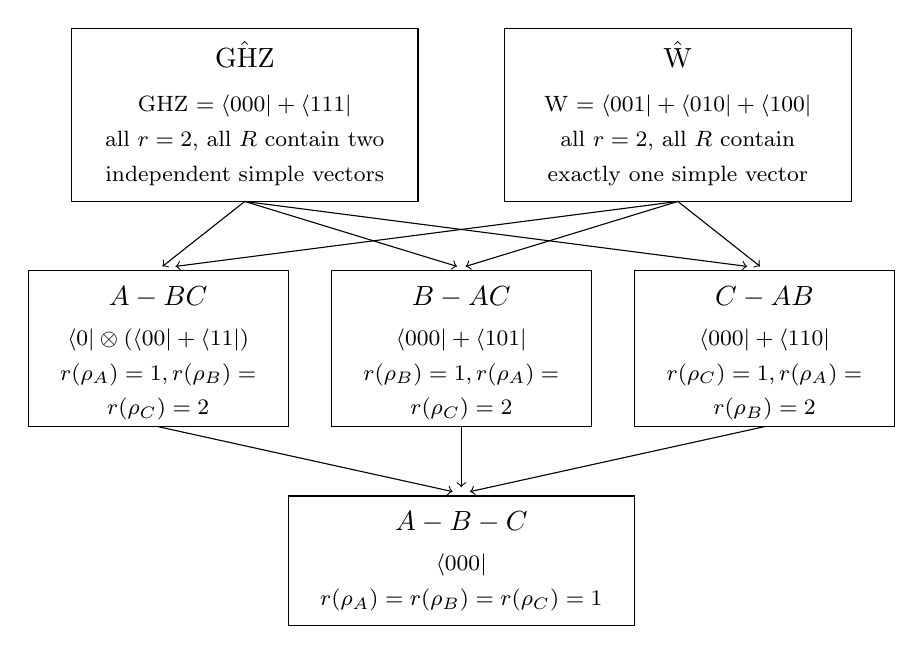
\begin{tikzpicture}[scale=1.1]
        \draw (-4.5,3) rectangle (-0.5,1);
        \node at (-2.5,2.7) {$\hat{\mathrm{GHZ}}$};
        \node at (-2.5,2.1) {\footnotesize{GHZ $= \langle 000\vert + \langle 111 \vert$}};
        \node at (-2.5,1.7) {\footnotesize{all $r =2$, all $R$ contain two}};
        \node at (-2.5,1.3) {\footnotesize{independent simple vectors}};
    
        \draw (0.5,3) rectangle (4.5,1);
        \node at (2.5,2.7) {$\hat{\mathrm{W}}$};
        \node at (2.5,2.1) {\footnotesize{W $= \langle 001\vert + \langle 010 \vert + \langle 100\vert$}};
        \node at (2.5,1.7) {\footnotesize{all $r =2$, all $R$ contain}};
        \node at (2.5,1.3) {\footnotesize{exactly one simple vector}};
    
        \draw (-5,0.2) rectangle (-2,-1.6);
        \node at (-3.5,-0.1) {$A - BC$};
        \node at (-3.5,-0.6) {\footnotesize{$\langle 0 \vert \otimes (\langle 00 \vert + \langle 11 \vert)$}};
        \node at (-3.5,-1) {\footnotesize{$r(\rho_A) = 1, r(\rho_B) =$}};
        \node at (-3.5,-1.4) {\footnotesize{$r(\rho_C) = 2$}};
    
        \draw (-1.5,0.2) rectangle (1.5,-1.6);
        \node at (0,-0.1) {$B - AC$};
        \node at (0,-0.6) {\footnotesize{$\langle 000 \vert + \langle 101 \vert$}};
        \node at (0,-1) {\footnotesize{$r(\rho_B) = 1, r(\rho_A) =$}};
        \node at (0,-1.4) {\footnotesize{$r(\rho_C) = 2$}};
    
        \draw (2,0.2) rectangle (5,-1.6);
        \node at (3.5,-0.1) {$C - AB$};
        \node at (3.5,-0.6) {\footnotesize{$\langle 000 \vert + \langle 110 \vert$}};
        \node at (3.5,-1) {\footnotesize{$r(\rho_C) = 1, r(\rho_A) =$}};
        \node at (3.5,-1.4) {\footnotesize{$r(\rho_B) = 2$}};
    
        \draw (-2,-2.4) rectangle (2,-3.9);
        \node at (0,-2.7) {$A - B - C$};
        \node at (0,-3.2) {\footnotesize{$\langle 000 \vert$}};
        \node at (0,-3.6) {\footnotesize{$r(\rho_A) = r(\rho_B) = r(\rho_C) = 1$}};

        \draw[<->] (-0.05,0.25) -- (-2.5,1) -- (-3.45,0.25);
        \draw[->] (-2.5,1) -- (3.3,0.25);
        \draw[<->] (0.05,0.25) -- (2.5,1) -- (3.45,0.25);
        \draw[->] (2.5,1) -- (-3.3,0.25);
        \draw[->] (3.5,-1.6) -- (0.1,-2.35);
        \draw[->] (0,-1.6) -- (0,-2.3);
        \draw[->] (-3.5,-1.6) -- (-0.1,-2.35);
    \end{tikzpicture}

\end{document}